\chapter{Quadrupole Moment}
\label{app:quadrupole}

\begin{figure}
	\centering
	\makebox[\textwidth]{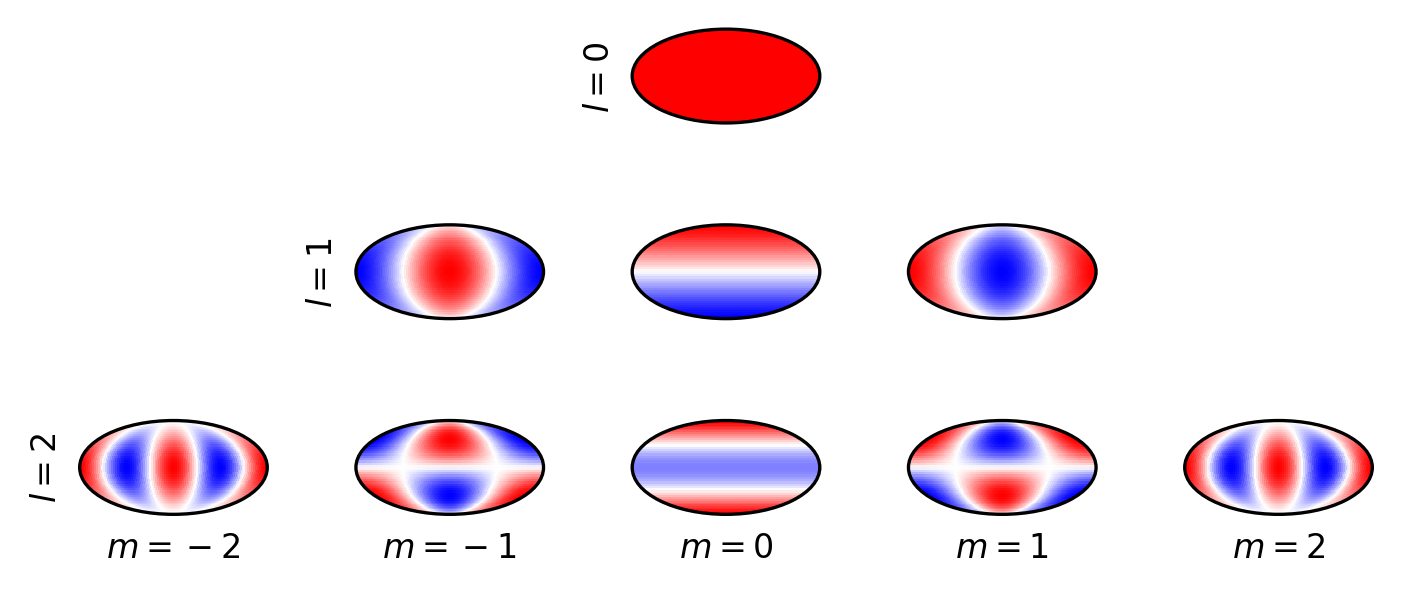
\includegraphics[width=12cm]{theory_of_gravitational_waves/images/spherical_harmonics/spherical_harmonics}}
	\caption{Visualization of the spherical harmonics up to $l=2$. The plots show the normalization of $\Re Y^m_l(\theta,\phi)$ on a Mollweide projection.}
	\label{fig:gravitational_waves:spherical_harmonics}
\end{figure}

In the transverse-traceless gauge, the quadrupole moment tensor takes the form,
\begin{equation}
	Q_{ij} = \int\mathrm{d}^3\vec{r}\,(3r_ir_j - \delta_{ij}r^2)T_{00}(t, \vec{r}).
\end{equation}
By expanding the energy density $T_{00}$ as
\begin{equation}
	T_{00}(t, \vec{r}) = \sum_l \sum_{m=-l}^l \rho_{lm}(t, r)Y^m_l(\theta, \phi)
\end{equation}
with the spherical harmonic functions $Y^m_l$ and coefficients $\rho_{lm}$, it can be shown that only the $l=2$ coefficients contribute to the quadrupole moment tensor.
This follows from the fact that $3r_ir_j - \delta_{ij}r^2$ can be expanded purely in $l=2$ spherical harmonics. That is,
\begin{equation}
	\label{eq:appendix:quadrupole}
	3r_ir_j - \delta_{ij}r^2 = r^2\sum_{m=-2}^{2}c_mY^m_{l=2},
\end{equation}
which will be verified later. Then, 
\begin{equation}
	Q_{ij} = \sum_{m'}\sum_{l,m}\tilde{c}_{m'}
	\int\mathrm{d}r\,r^4\rho_{lm}(t, r)\,
	\int\mathrm{d}\Omega\,
	(Y_{l'=2}^{m'})^* Y_{l}^{m},
\end{equation}
making use of $(Y_l^m)^* = (-1)^mY^{-m}_l$, and defining $\tilde{c}_m = (-1)^{-m}c_{-m}$.
The orthonormality of the spherical harmonics,
\begin{equation}
	\int\mathrm{d}\Omega\,(Y^{m'}_{l'})^*Y^m_l = \delta_{ll'}\delta_{mm'},
\end{equation}
yields
\begin{equation}
	Q_{ij} = \sum_{m}\tilde{c}_m\int\mathrm{d}r\,r^4\rho_{l=2,m}(t, r).
\end{equation}
This shows that the quadrupole moment tensor is non-vanishing only if the mass distribution has a non-zero $l=2$ spherical harmonic contribution. From this it is obvious that spherically symmetric ($l=0$) systems do not radiate. See Fig.~\ref{fig:gravitational_waves:spherical_harmonics} for a visualization of the spherical harmonics. The $l=2$ distributions are peanut-shaped. Prime examples of time-varying systems with $l=2$ mass distributions are orbiting binary systems.

Eq.~\ref{eq:appendix:quadrupole} can be written out explicitly as, 
% chat gpt says to put 3 instead of 2 for 3x²-r² and 3y²-r²
\begin{align}
	3x^2 - r^2 &= 3\sqrt\frac{2\pi}{15}r^2(Y^2_2+Y^{-2}_2) - 2\sqrt\frac{\pi}{5}r^2Y^0_2, \\
	3y^2 - r^2 &= -3\sqrt\frac{2\pi}{15}r^2(Y^2_2+Y^{-2}_2) - 2\sqrt\frac{\pi}{5}r^2Y^0_2, \\
	3z^2 - r^2 &= 4\sqrt\frac{\pi}{5}r^2Y^0_2, \\
	xy &= -i\sqrt{\frac{2\pi}{15}}r^2(Y^2_2-Y^{-2}_2), \\
	yz &= i\sqrt{\frac{2\pi}{15}}r^2(Y_2^1+Y_2^{-1}), \\
	zx &= -\sqrt\frac{2\pi}{15}r^2(Y_2^1 - Y_2^{-1}).
\end{align}
This can be verified from the $l=2$ harmonics:
\begin{alignat}{2}
	Y_{2}^{-2}(\theta,\varphi)
	& = \frac{1}{4}\sqrt\frac{15}{2\pi}\e^{-2i\varphi}\sin^{2}\theta
	&& = \frac{1}{4}\sqrt\frac{15}{2\pi}\frac{(x - iy)^2}{r^{2}}, \\
	Y_{2}^{-1}(\theta,\varphi)
	& = \frac{1}{2}\sqrt\frac{15}{2\pi}\e^{-i\varphi}\sin\theta\cos\theta
	&& = \frac{1}{2}\sqrt\frac{15}{2\pi}\frac{(x - iy)z}{r^{2}}, \\
	Y_{2}^{ 0}(\theta,\varphi)
	& = \frac{1}{4}\sqrt\frac{5}{\pi}(3\cos^{2}\theta-1)
	&& = \frac{1}{4}\sqrt\frac{5}{\pi}{(3z^{2}-r^{2})\over r^{2}}, \\
	Y_{2}^{ 1}(\theta,\varphi)
	& = -\frac{1}{2}\sqrt\frac{15}{2\pi}\e^{  i\varphi}\sin\theta\cos\theta
	&& = -\frac{1}{2}\sqrt\frac{15}{2\pi}\frac{(x + iy) z}{r^{2}}, \\
	Y_{2}^{ 2}(\theta,\varphi)
	& = \frac{1}{4}\sqrt\frac{15}{2\pi}\e^{ 2i\varphi}\sin^{2}\theta
	&& = \frac{1}{4}\sqrt\frac{15}{2\pi}\frac{(x + iy)^2}{r^{2}}.
\end{alignat}
